%%% Dichiarazione dei pacchetti standard.
\documentclass{beamer}
\usepackage[utf8]{inputenc}
\usepackage[italian]{babel}
\usepackage{graphicx}
\usepackage{wrapfig}
\usepackage{amsfonts}
%\usepackage[square, numbers, comma, sort&compress]{natbib}  % Use the
                                % "Natbib" style for the references in
                                % the Bibliography

%%% Personalizzazione del layout---articolata su cinque livelli.
%\usetheme{split}        % layout complessivo. 
%\usetheme{Goettingen}        % layout complessivo. 
%\usetheme{CambridgeUS}        % layout complessivo. 
%\usetheme{Boadilla}        % layout complessivo. 
%\usetheme{Montpellier}        % layout complessivo. 
%\usetheme{Warsaw}        % layout complessivo. 
%\usetheme{Pittsburgh}        % layout complessivo. 
\usetheme{Hannover}        % layout complessivo. 

\useinnertheme{default} % layout interno.
\useoutertheme{default} % layout esterno.
\usecolortheme{default} % schema di colori.
\usefonttheme{default}  % schema dei font.
% Inutile dire che se volete tutti i default, potete risparmiarvi gli ultimi
% quattro comandi. 
\definecolor{jgreen}{RGB}{0,92,40}
\definecolor{jyellow}{RGB}{211,168,0}
\definecolor{jred}{RGB}{153,32,0}
\beamertemplatenavigationsymbolsempty 
\setbeamercolor{sidebar}{bg=jgreen}
\setbeamercolor{section in sidebar}{fg=yellow}
\setbeamercolor{title in sidebar}{fg=white}
\setbeamercolor{author in sidebar}{fg=jred}
\setbeamercolor{frametitle}{fg=jgreen}
\setbeamercolor{title}{fg=jgreen}
\setbeamercolor{item}{fg=jgreen}

%%% Titolo e autore.

\title{Reti federate eventualmente connesse}
\subtitle{Architettura e prototipo per la Rete Mocambos}
\author{Vincenzo Tozzi}
\institute{Universit\`a degli Studi di Firenze - Corso di Laurea in Informatica}
\date{23 aprile 2012}

\begin{document}

% Local background must be enclosed by curly braces for grouping.
{
\usebackgroundtemplate{
  \hspace{0.02cm}
  
\includegraphics[width=.3\textwidth]{./Figure/logoUNIFI.pdf}
}%
\begin{frame}
  \titlepage
\end{frame}
}

% \section[Sommario]{}
% \begin{frame}
%   \tableofcontents
% \end{frame}

\section{Digital divide e libertà tecnologica}

\begin{frame}

  \frametitle{\emph{Digital divide} in Brasile}
  Popolazione con accesso ad Internet in Brasile\footnote{Fonte: intervista al Segretario Esecutivo del Ministero delle
    Comunicazioni, Cesar Alvarez, su dati IBGE 2009.}:
  \begin{itemize}
    \item $\sim$ 30\% della popolazione
    \item $\sim$ 6\% della popolazione in area rurale  
  \end{itemize}
    
\end{frame}


{
\usebackgroundtemplate{
%  \hspace{2cm}
  \begin{picture}(0,0)\put(130,-270)
    {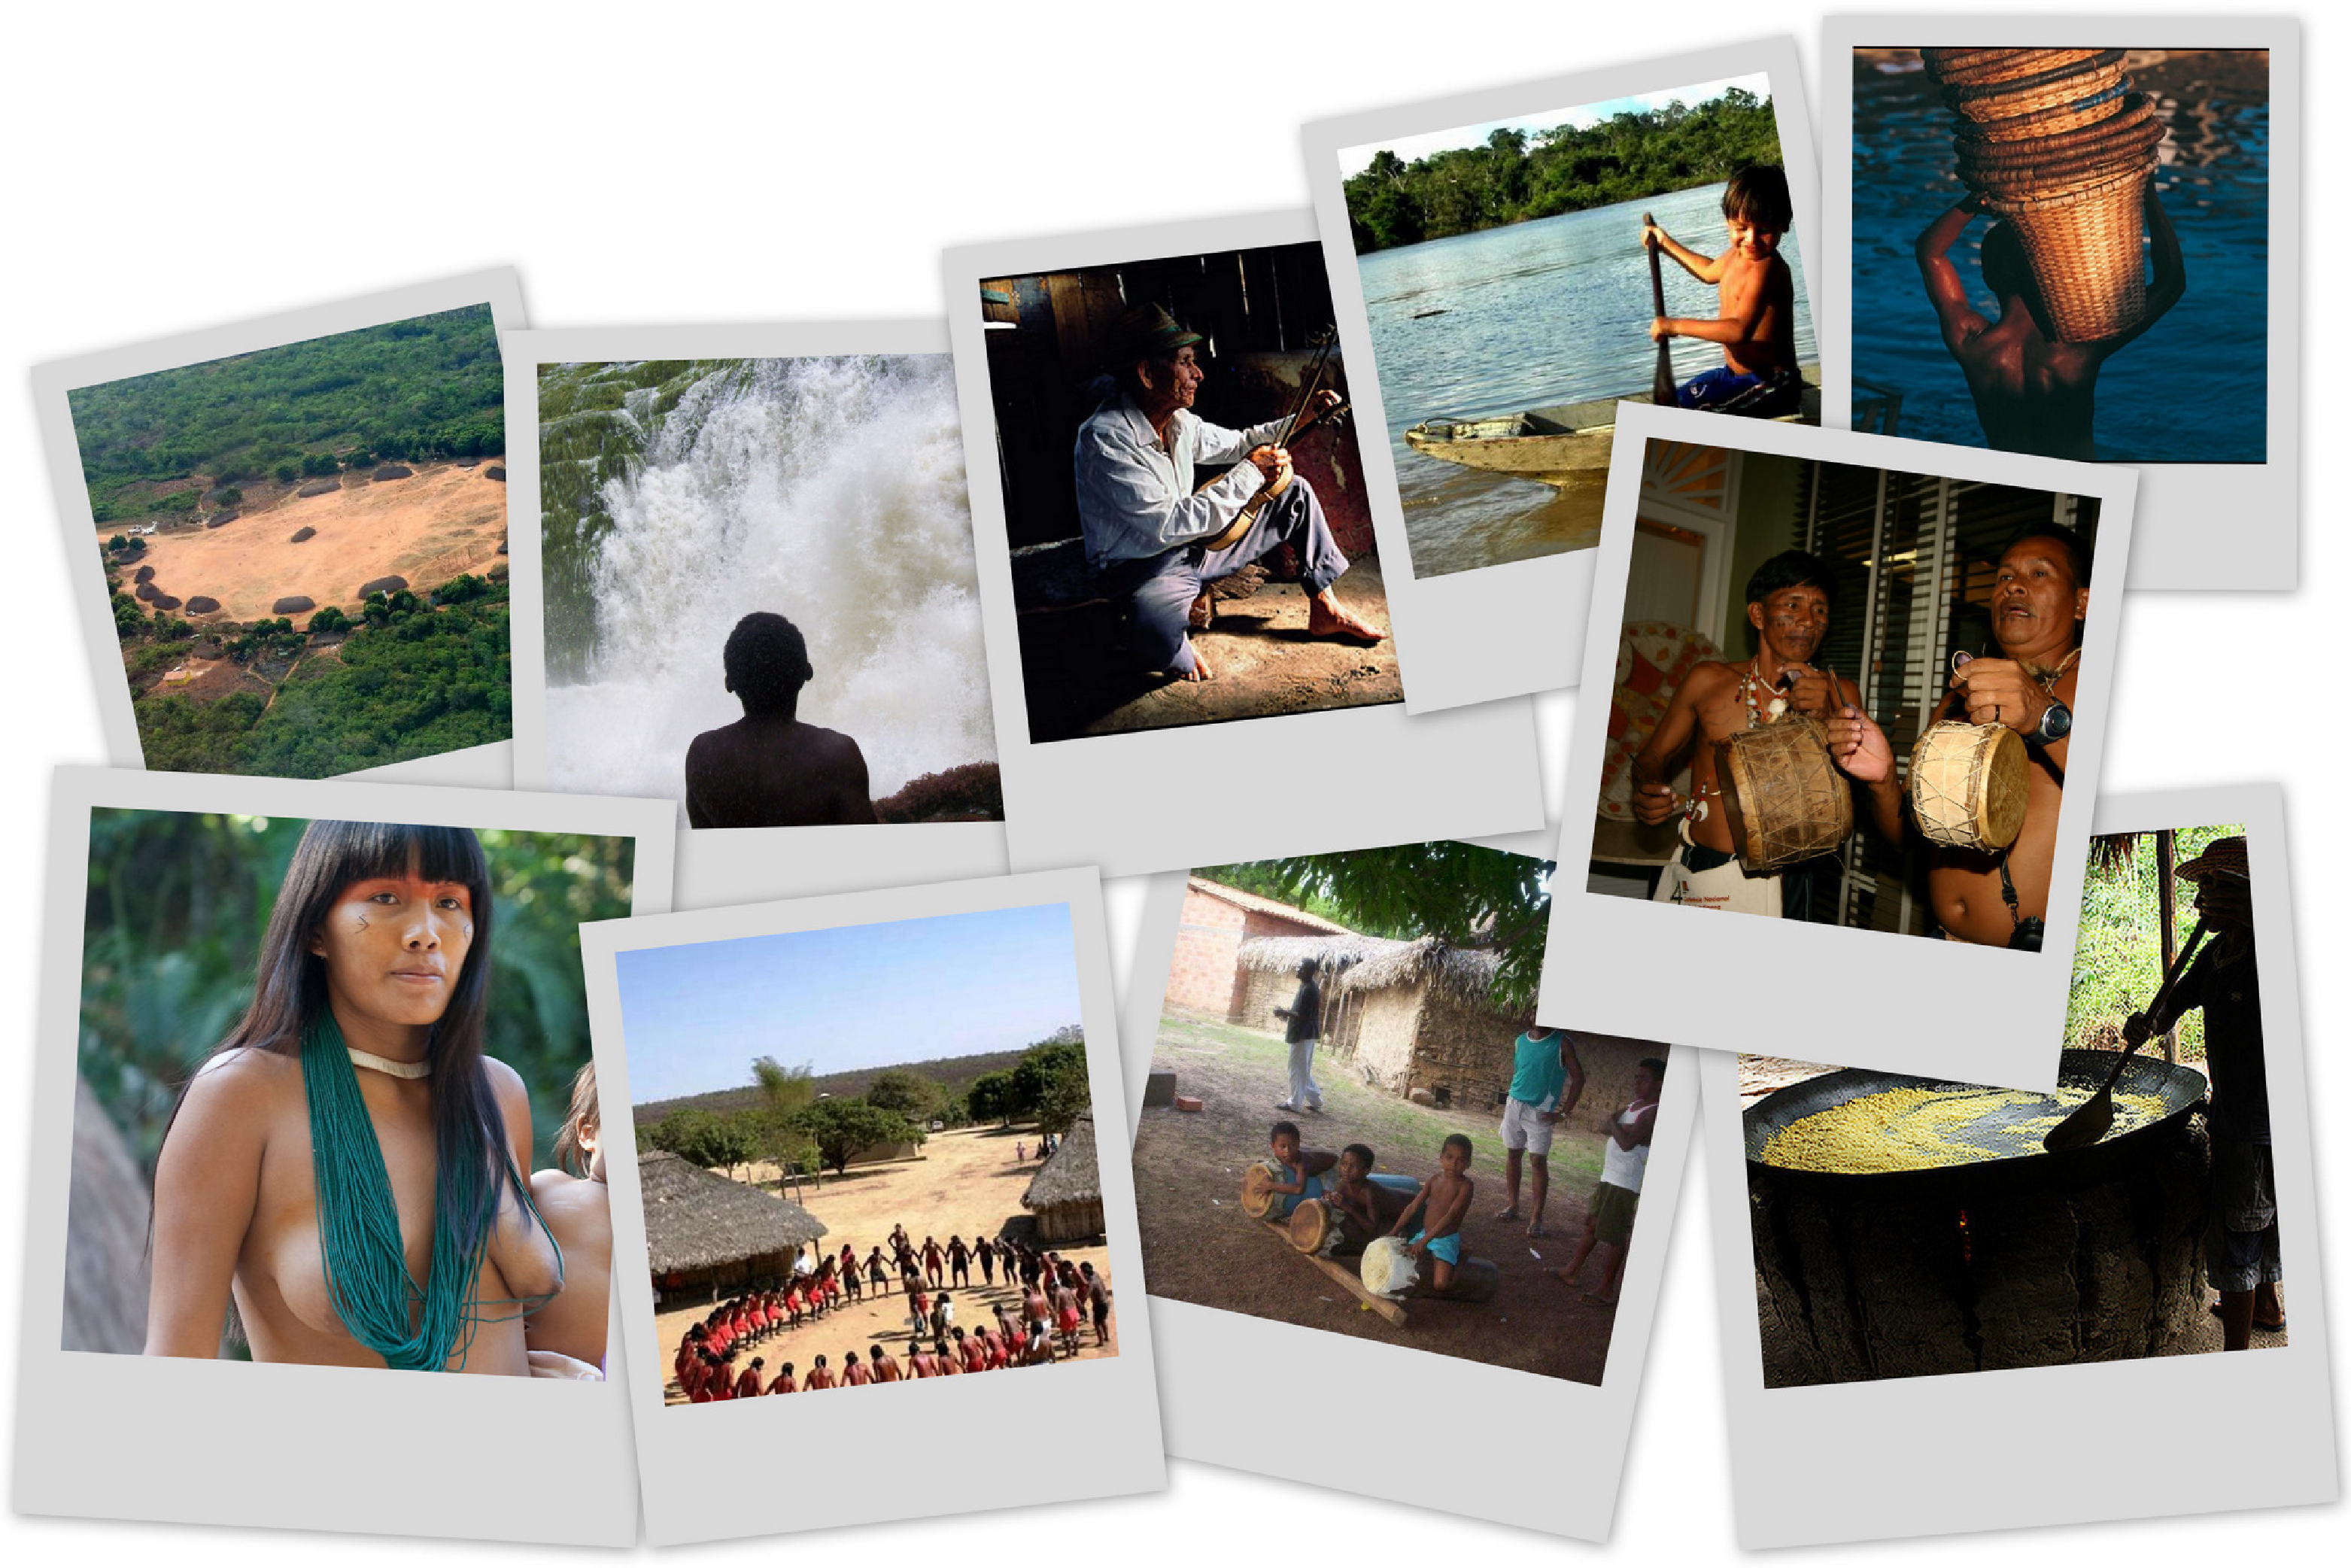
\includegraphics[width=0.8\textwidth]{./Figure/diversidade.pdf}}
  \end{picture}}

\begin{frame}

  \frametitle{Brasile: Uno, nessuno e centomila}
  Il Brasile è un paese di dimensione continentale dove convivono
  molte culture in ambienti e contesti molto diversi. 
  \begin{itemize}
  \item Indios
  \item Quilombola
  \item Caiçaras
  \item Riberinhos
  \item \ldots
  \end{itemize}

\end{frame}

}

\begin{frame}

  \frametitle{Come si affronta il digital divide?}
  \begin{itemize}
    \item Alfabetizzazione informatica
    \item Accesso a internet
    \item e poi\ldots
    \item Ricerca e sviluppo?
    \end{itemize}

 \end{frame}

\begin{frame}

  \frametitle{Neutralità tecnologica}

  \begin{quote}
    ``Siamo portati a pensare al mezzo come neutrale, ma se prendiamo
    ad esempio i principali e più diffusi mezzi di comunicazione, le
    lingue, possiamo intuire come queste non siano interscambiabili
    essendo l'espressione delle culture e delle società che le usano e
    le vivono.''
  \end{quote}
  
\end{frame}


\begin{frame}
  \frametitle{Internet, autonomia e libertà tecnologica}
  \framesubtitle{Dagli RFC\ldots}
  \begin{quote}
  ``Internet è nata dal confronto aperto tra i responsabili di diverse
  reti, uniti dalla volontà di connettere le loro differenti
  realtà. La nascita di nuovi servizi, per queste reti eterogenee, era
  basata sulla discussione e il confronto.'' 
\end{quote}

\end{frame}

\begin{frame}
  \frametitle{Internet, autonomia e libertà tecnologica}
  \framesubtitle{\ldots ai ToS/API/Cloud}
  \begin{quote}
  ``Negli ultimi anni la diffusione della banda larga, ma sopratutto
  strategie come quella adottata da Google, hanno  trasformato il 
  concetto stesso di internet che da rete globale di reti eterogenee,
  diventa principalmente una rete per la globalizzazione di servizi
  fortemente centralizzati e uniformati.'' 
  \end{quote}
\end{frame}

\begin{frame}
  \frametitle{Internet, autonomia e libertà tecnologica}
  \framesubtitle{\ldots ai ToS/API/Cloud}
  \begin{quote}
    ``Secondo la società di consulenza Gartner, nel 2016, tutte le
    compagnie contemplate dal \emph{Forbes Global 2000} faranno uso di
    soluzioni \emph{cloud} \footnote{Tratto dall'articolo: ``Six global trends
      shaping the business world'', del 2011, pubblicato sulla rivista EY
      Insights di Ernst \& Young}.''
  \end{quote}
\end{frame}

\begin{frame}
  \frametitle{Dalle maestranze informatiche\ldots}
  \framesubtitle{\ldots ai nuovi operai}
  \begin{quotation}
    ``\ldots un tempo lo sviluppo seguiva un modello \emph{bottom up}, per
    cui le maestranze informatiche sviluppavano sistemi ad hoc per le
    esigenze locali, per poi in seguito aprire una discussione in
    rete, con i loro corrispettivi, per definire dei protocolli
    standard e mettere in comunicazione il tutto.

    Oggi si passa ad un modello di sviluppo \emph{top down}, per cui
    nuovi servizi vengono lanciati basandosi su indagini di mercato e
    test su campioni di utenti.''
  \end{quotation}
\end{frame}


\section{Reti federate eventualmente connesse}

\begin{frame}
  \frametitle{La Rete Mocambos}
  \begin{itemize}
    \item Più di 200 comunità rurali sparse su tutto il territorio
      nazionale, principalmente in zone amene
    \item Comunità di matrice africana (quilombos) e indigena (aldeias)
    \item Uso critico e autonomo di TIC
    \item Banda disponibile limitata (connessioni satellitari 512/128 Kbps)
    \end{itemize}
\end{frame}

\begin{frame}
  \frametitle{La Rete Mocambos}
  \framesubtitle{Mappa delle comunità}
	\begin{figure}
		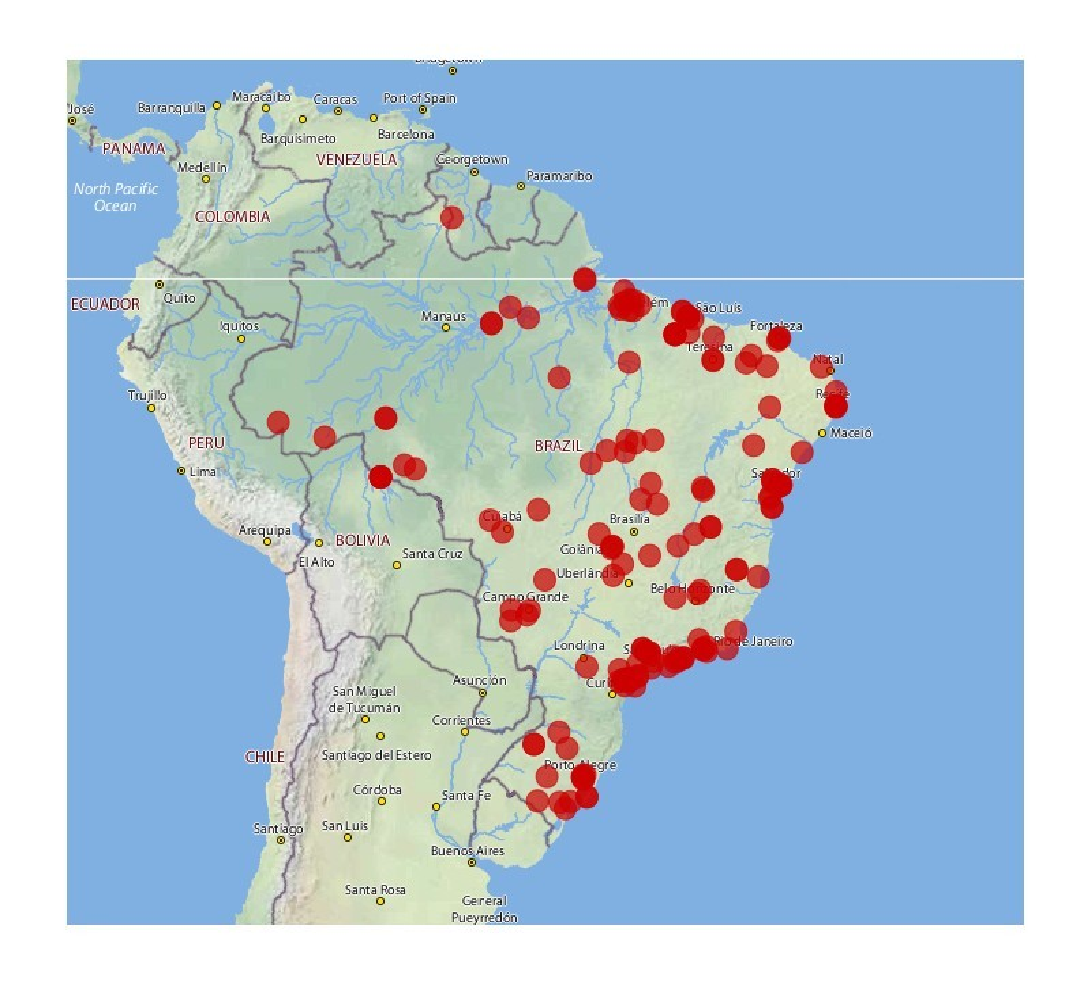
\includegraphics[height=0.7\textheight]{./Figure/MappaRedeMocambos.pdf}
	\end{figure}
\end{frame}




\begin{frame}
  \frametitle{Reti federate eventualmente connesse}
  \begin{quote}
    ``una rete federata basata su connessioni non sempre disponibili,
    quali le connessioni satellitari, con l'esigenza di mantenere i
    servizi federati attivi, anche in assenza di comunicazione. I
    servizi federati sono inoltre ottimizzati per la resilienza del
    sistema e la riduzione del traffico di rete esterno, attraverso
    strategie di replicazione, sincronizzazione e memorizzazione dei
    dati sull'infrastruttura logica/fisica locale.''
    \end{quote}
\end{frame}


% Local background must be enclosed by curly braces for grouping.
{
%\usebackgroundtemplate{\includegraphics[width=.4\textwidth]{include/pista.jpg}}%
\begin{frame}
  \frametitle{Reti federate eventualmente connesse}
  \framesubtitle{Tecnologie e strumenti utili}
  \begin{itemize}
    \item LDAP
    \item XMPP
    \item OpenID
    \item OAuth
    \item Django / Ruby On Rails
    \item git / git-annex
    \item rsync
    \end{itemize}
\end{frame}
}


\section{Un'architettura per la Rete Mocambos}

\begin{frame}
  \frametitle{Un'architettura per la Rete Mocambos}
  \framesubtitle{Specifica dei requisiti}
  \begin{itemize}
    \item Identità di rete
    \item Autenticazione decentrata
    \item Sincronizzazione
    \item Riproducibilità
    \item Manutenzione
    \item Sviluppo
    \end{itemize}

\end{frame}

\begin{frame}
  \frametitle{Un'architettura per la Rete Mocambos}
  \framesubtitle{Strumenti e pratiche per lo sviluppo}
  \begin{itemize}
    \item Documentazione e ``versionamento'': wiki, git
    \item Sistema operativo: Debian e Ubuntu
    \item Linguaggi di programmazione: Python, shell script
    \item Virtualizzazione: Virtualbox, Virtualenv
    \end{itemize}

\end{frame}

\begin{frame}
  \frametitle{Un'architettura per la Rete Mocambos}
  \framesubtitle{Architettura di base}
	\begin{figure}
		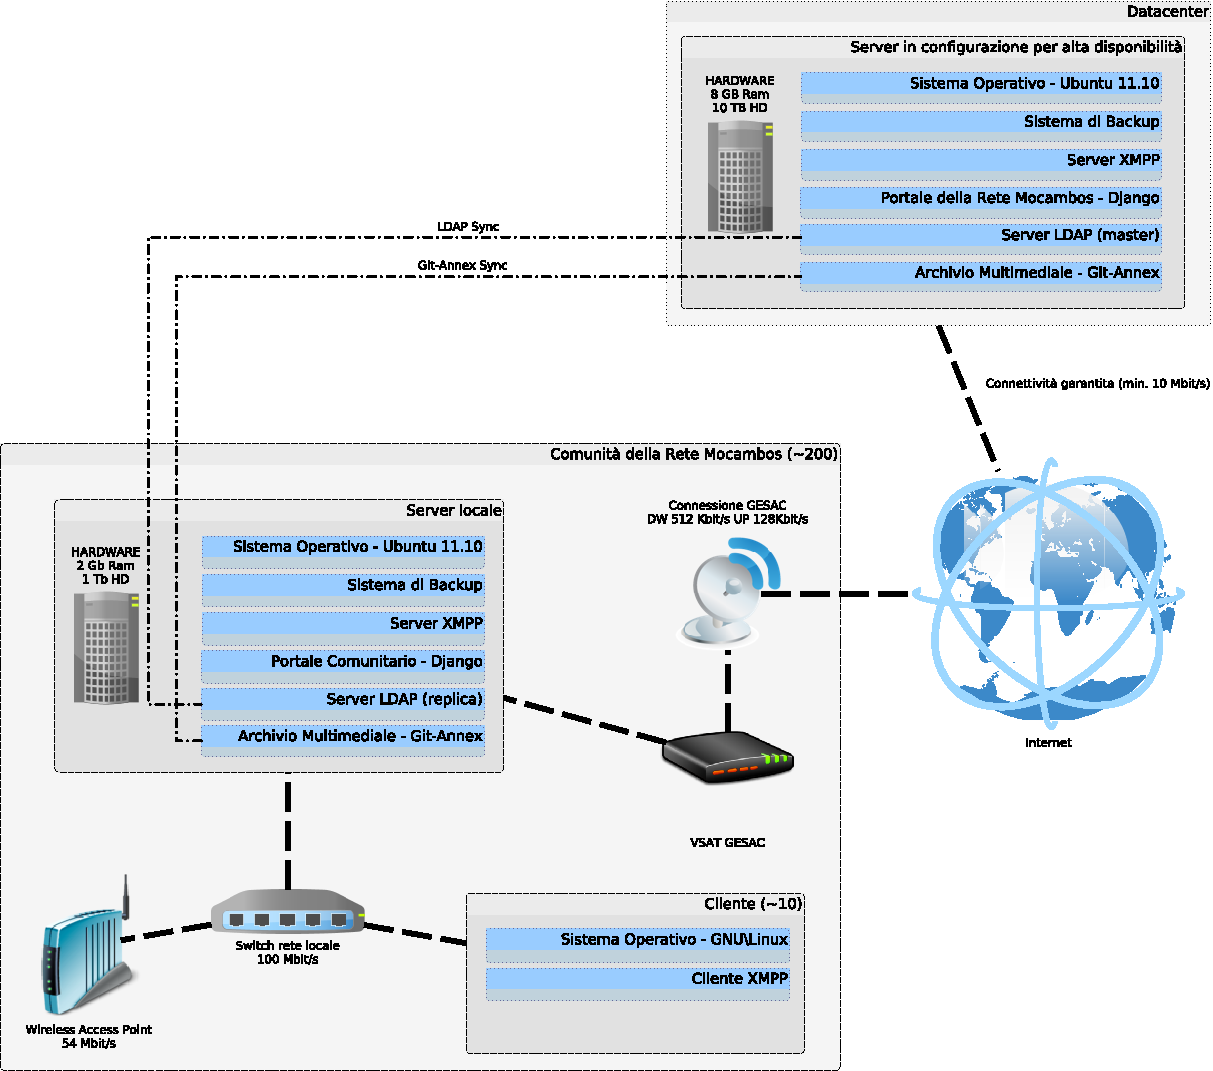
\includegraphics[height=0.7\textheight]{./Figure/SchemaServer_ReteMocambos-crop.pdf}
	\end{figure}
\end{frame}

\section{Un prototipo di servizio federato}

\begin{frame}
  \frametitle{Un prototipo di servizio federato}
  \framesubtitle{Sistema di pubblicazione e diffusione di contenuti multimediali}
	\begin{figure}
		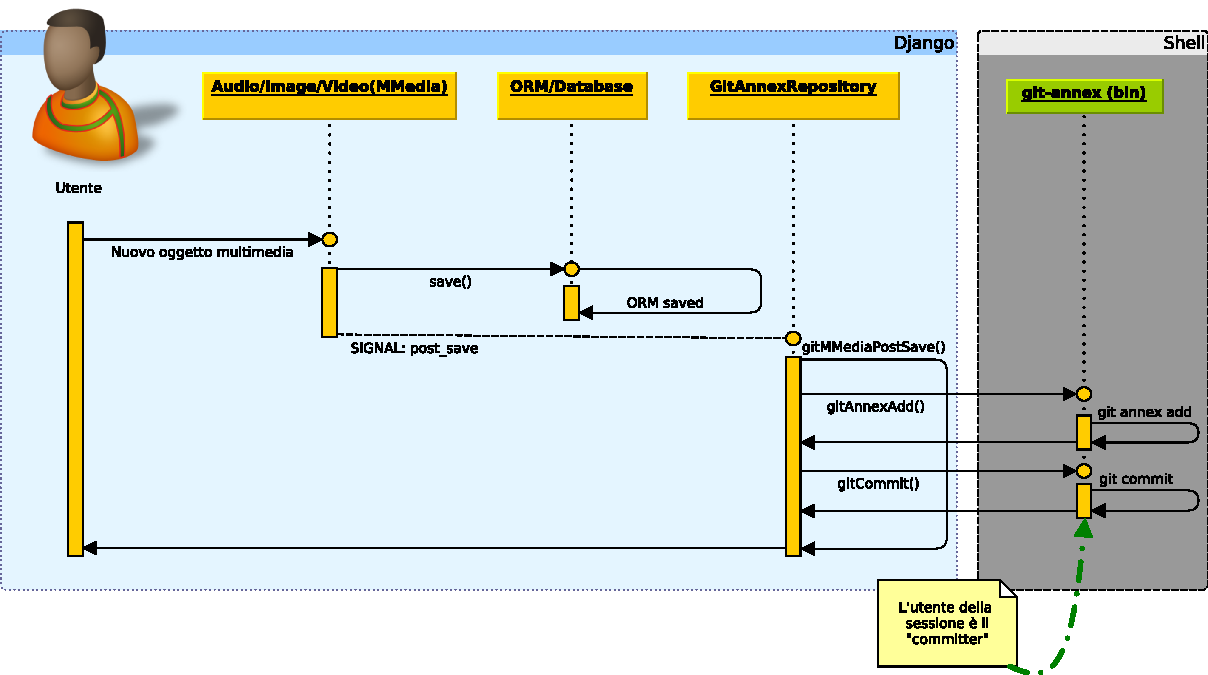
\includegraphics[width=\textwidth]{./Figure/SequenceDiagram_NuovoOggetto-crop.pdf}
	\end{figure}
\end{frame}

\begin{frame}
  \frametitle{Un prototipo di servizio federato}
  \framesubtitle{Archivio multimediale}
\emph{git-annex} supporta:
\begin{itemize}
\item localizzazione delle copie (\emph{location tracking})
\item scaricamento selettivo dei contenuti
\item gestione della fiducia dei \emph{repository}
\item gestione del numero di repliche minimo
\item vari \emph{backend} per le chiavi (SHA, WORM)
\item vari \emph{backend} per i contenuti/valori (BUP, rsync, web, S3)
\end{itemize}

\end{frame}

\section{Conclusioni e sviluppi futuri}

\begin{frame}
 \frametitle{Conclusioni e sviluppi futuri}
  \begin{quote}
    ``L'architettura e il prototipo sviluppati sono in corso di
    implementazione, su scala ridotta, a partire dalle comunità più
    strutturate e che fungono già da poli regionali, chiamati Nuclei
    di Formazione Continua, che sono attualmente dieci,
    geograficamente ben distribuiti sul territorio nazionale
    brasiliano.''
  \end{quote}
\end{frame}

\begin{frame}
 \frametitle{Conclusioni e sviluppi futuri}
  \framesubtitle{Risultati\ldots}
  Funzionalità implementate:
  \begin{itemize}
  \item autenticazione LDAP (con gestione basica dei gruppi)
  \item creazione e upload di contenuti audio, immagini e video
  \item distribuzione tramite \emph{git-annex}
  \item sincronizzazione degli oggetti sui portali django (ricreando
    gli oggetti relativi ai contenuti distribuiti via
    \emph{git-annex})
  \end{itemize}
\end{frame}
  
\begin{frame}
 \frametitle{Conclusioni e sviluppi futuri}
  \framesubtitle{\ldots e prossime versioni}
 
  Da implementare:
  \begin{itemize}
  \item trasferimento selettivo dei contenuti/valori basato sull'uso
    statistico o su richiesta
  \item sviluppo di in interfaccia di visualizzazione e pubblicazione
    per l'utente finale
  \item gestione del DIT dell'LDAP tramite script e/o portale
  \end{itemize}
\end{frame}

\begin{frame}
 \frametitle{Partner}
 La Rete Mocambos conta con l'appoggio di altre reti, collettivi e istituzioni
  
  \begin{itemize}
  \item Pontos de Cultura 
  \item Metareciclagem
  \item Rete Dyne 
  \item \ldots
  \end{itemize}
  
  Partner istituzionali:
  \begin{itemize}
  \item GESAC
  \item Telecentros.BR
  \item Secretaria de Políticas de Promoção da Igualdade Racial da
    Presidência da República
  \item Unicamp 
  \item \ldots
  \end{itemize}
  
\end{frame}

\section{Extra}

\begin{frame}
  \frametitle{}
 \end{frame}

\begin{frame}
 \frametitle{Fine}
 \begin{center}
   \huge Grazie per l'attenzione! :) \\
   \vfill
   \large  
   Vincenzo Tozzi \\
   \normalsize
   vince@mocambos.net
   \vfill
   \begin{figure}[htb]
     \begin{minipage}[c]{0.10\textwidth}
       
\includegraphics[width=\textwidth]{./Figure/NPDD.pdf}
  \end{minipage}
  \begin{minipage}[c]{0.60\textwidth}
    \footnotesize
    Nucleo de Pesquisa e Desenvolvimento Digital \\*
    Casa de Cultura Tainã/Rede Mocambos\\*
    http://wiki.mocambos.net/wiki/NPDD
  \end{minipage}

\end{figure}
\end{center}
\end{frame}




\end{document}
